\documentclass[tikz,border=10pt]{standalone}
% Scale: s = 0.008511 cm/px, origin at C, y flipped
\begin{document}
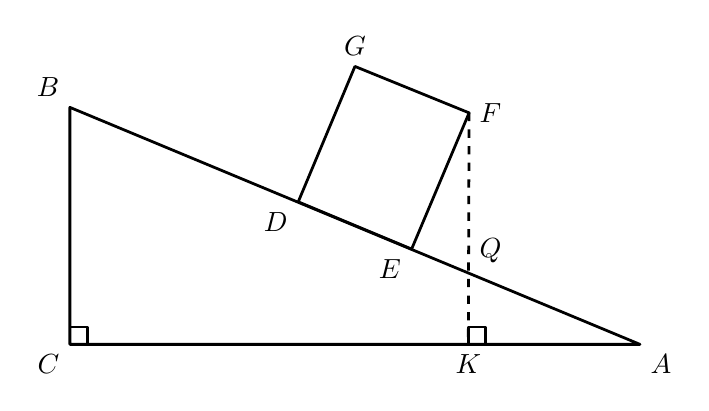
\begin{tikzpicture}[line join=round, line width=1.0pt,
  lbl/.style={font=\fontsize{10}{12}\selectfont}]

% Named points (converted from image px)
\coordinate (C) at (0,0);
\coordinate (A) at (7.24,0);
\coordinate (B) at (0,3.01);
\coordinate (K) at (5.06,0);
\coordinate (D) at (2.90,1.81);
\coordinate (E) at (4.34,1.21);
\coordinate (F) at (5.07,2.94);
\coordinate (G) at (3.62,3.53);
\coordinate (Q) at (5.07,0.90);

% Triangle
\draw (B) -- (C) -- (A) -- cycle;

% Rectangle DGFE (solid)
\draw (D) -- (G) -- (F) -- (E) -- cycle;

% Dashed altitude F to K (through Q)
\draw[dashed] (F) -- (K);

% Right-angle marks (one each)
% Mark at C (unchanged)
\draw (0.22,0) -- (0.22,0.22) -- (0,0.22);
% Mark at K: closed square (up and right of K, 0.22 units = 26 px)
\draw (K) ++(0,0) -- ++(0,0.22) -- ++(0.22,0) -- ++(0,-0.22) -- cycle;

% Labels
\node[lbl, above left] at (B) {$B$};
\node[lbl, below left] at (C) {$C$};
\node[lbl, below right] at (A) {$A$};
\node[lbl, below] at (K) {$K$};
\node[lbl, above] at (G) {$G$};
\node[lbl, right] at (F) {$F$};
\node[lbl, below left] at (D) {$D$};
\node[lbl, below left] at (E) {$E$};
\node[lbl, above right] at (Q) {$Q$};

\end{tikzpicture}
\end{document}